\chapter{Proposta}

%=====================================================

Como discutido na seção anterior, é possível treinar um modelo de classificação generalista o suficiente capaz de alcançar resultados de em média 95\% de acurácia nos cenários de validação cruzada entre datasets, sem a necessidade de algum ajuste ou treinamento para um cenário específico \citep{hochuli-2}. Porém, resultados ainda melhores, em média 97\% de acurácia, podem ser alcançados ao se realizar um ajuste fino em um modelo generalista com poucos dados rotulados de cenários específicos \citep{hochuli-1}.

Ainda assim, a dificuldade e esforço em se obter e rotular dados persiste, sendo necessário realizar esse trabalho de coleta a cada novo cenário em que se desejar um modelo com a melhor performance possível. Uma forma de tentar contornar esse problema é a utilização de dados sintéticos no treinamento, mais especificamente imagens sintéticas, já que, além de ser possível gerar as mais diversas condições climáticas e de iluminação, milhões de imagens rotuladas podem ser geradas em minutos, podendo ser usadas para substituir imagens reais ou em conjunto com elas \citep{objectPose} \citep{domain-random} \citep{fully-synthetic-training} \citep{synthetic-pedestrians}.

Na seção anterior vimos que em \citet{synthetic-parking2} ótimos resultados foram atingidos na classificação de vagas utilizando de imagens sintéticas geradas a partir de um ambiente de simulação altamente fiel ao cenário real, com condições de iluminação, câmera e clima altamente realistas. Porém, construir esse ambiente simulado de alta fidelidade é mais trabalhoso que a coleta e rotulação de imagens reais de um cenário específico, não tendo ganhos em performance suficientes para justificar a utilização desse método. Em \citet{domain-random}, podemos ver que imagens sintéticas randomizadas e de baixa fidelidade à realidade podem alcançar resultados comparáveis a de imagens reais ao serem utilizadas em modelos de Deep Learning, sendo necessário um esforço consideravelmente pequeno para serem geradas. Com isso, a proposta deste trabalho é utilizar deste método de geração de dados sintéticos para responder 2 perguntas de pesquisa:
\begin{itemize}
    \item P1 - Qual o impacto das imagens sintéticas de baixa fidelidade na eficiência dos modelos estado da arte de classificação de vagas de estacionamento em cenários cruzados?
    \item P2 - É possível superar o estado da arte treinando os modelos somente com imagens sintéticas de baixa fidelidade?
\end{itemize}

O processo de aprendizado por transferência foi utilizado para o treinamento dos modelos e realização dos experimentos. O aprendizado por transferência usa um modelo base generalista como extrator de características, e uma camada de classificação final é incluída e treinada com as bases disponíveis para a afinação do modelo. Esse processo é simples e não necessita de muita capacidade computacional, sendo uma boa escolha dado o objetivo de diminuir os esforços. As próximas sub-seções fornecem uma explicação detalhada do processo de geração das imagens sintéticas e do modelo base e parâmetros escolhidos para o processo de aprendizado por transferência.

\section{Geração dos dados sintéticos}

A ferramenta de simulação que foi utilizada é a engine de jogos Unity5, em conjunto com o pacote Unity Perception \citep{unity-perception}. Esse pacote oferece diversas ferramentas de aleatorização do ambiente e possibilita a construção de um ambiente de simulação tanto de alta como baixa fidelidade. As imagens são capturadas automaticamente e as informações de contexto para rotulação são geradas automaticamente por meio da visão de uma câmera que pode ser posicionada de qualquer maneira em qualquer angulação. 

Para o ambiente simulado de baixa fidelidade neste trabalho, um script de aleatorização para as vagas do estacionamento e espaçamento entre elas foi criado e um conjunto de texturas para o chão e modelos 3D de carros e árvores foram selecionados. Primeiro seleciona-se a posição da câmera e o número de iterações da execução. Cada iteração gera uma imagem com informações de contexto e as informações para segmentação das vagas e rotulação como ocupada ou livre são geradas automaticamente. Cada iteração segue os seguintes passos:
\begin{itemize}
    \item Uma textura é escolhida e aplicada ao chão do ambiente.
    \item O script define as fileiras de vagas, suas posições, espaçamento entre as vagas e a rotação das mesmas. A cada 100 iterações, a posição de todas as vagas é rotacionada em 15 graus.
    \item Os carros são adicionados à cena. Cada vaga recebe ou não um carro, com uma probabilidade de 50\% entre ocupada ou livre.
    \item A posição e quantidade de árvores é selecionada e as árvores são adicionadas à cena aleatoriamente.
    \item Ajusta-se a posição e intensidade da luz, mudando cor e temperatura e também o clima. Isso gera ambientes que simulam climas ensolarados, chuvosos e também possibilita capturas que simulam horários como tarde, noite e dia.
    \item A imagem é capturada pela câmera e as informações de contexto são registradas.
\end{itemize}

Foram geradas diversas bases de imagens, cada uma simulando a posição e parâmetros de câmera de cada sub-base disponível nas bases CNRPark-EXT \citet{cnrpark} e PKLot \citep{pklot2}. No total, 12 diferentes bases de imagens foram geradas. O número de iterações selecionado foi o de 1500, cada iteração gerando uma imagem sintética, ou seja, cada base possui 1500 imagens do estacionamento completo e cerca de 20000 imagens das vagas segmentadas e rotuladas. A tabela \ref{tab:tabela-quantidades} mostra a relação de quantidade de imagens segmentadas para cada base.

\begin{table}[!htp]
    \centering
    \caption{Relação de quantidade de imagens sintéticas segmentadas}
    \label{tab:tabela-quantidades}
    \begin{tabular}{|c|ccc|}
    \cline{2-4}
    \multicolumn{1}{c|}{}& Empty & Occupied & Total \\
    \hline
    \texttt{CNR-cam1} & 14495 & 14605 & 29100 \\
    \hline
    \texttt{CNR-cam2} & 5429 & 5371 & 10800 \\
    \hline
    \texttt{CNR-cam3} & 9533 & 9667 & 19200 \\
    \hline
    \texttt{CNR-cam4} & 12158 & 12542 & 24700 \\
    \hline
    \texttt{CNR-cam5} & 15558 & 15642 & 31200 \\
    \hline
    \texttt{CNR-cam6} & 9027 & 9073 & 18100 \\
    \hline
    \texttt{CNR-cam7} & 12332 & 12168 & 24500 \\
    \hline
    \texttt{CNR-cam8} & 11434 & 11066 & 22500 \\
    \hline
    \texttt{CNR-cam9} & 8245 & 8255 & 16500 \\
    \hline
    \texttt{PKLot-UFPR04} & 18713 & 18787 & 37500 \\
    \hline
    \texttt{PKLot-UFPR05} & 9433 & 9567 & 19000 \\
    \hline
    \texttt{PKLot-PUCPR} & 35994 & 36106 & 72100 \\
    \hline
    \end{tabular}
\end{table}

O programa open source Fspy \citep{fspy} foi utilizado para coletar a posição e parâmetros da câmera de cada sub-base. A  figura \ref{fig:comparacao-ufpr04} mostra uma comparação entre a primeira e a milésima iteração da base de dados com os parâmetros da UFPR04.
% Figura 1 comparando imagens sintéticas UFPR04
\begin{figure}[!htb]
    \centering
    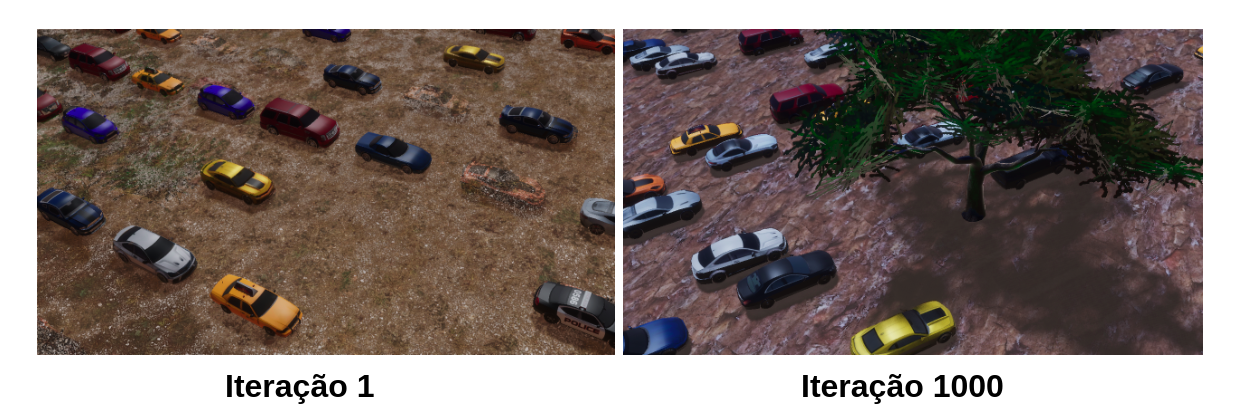
\includegraphics[width=15cm]{/home/eckermann/college/syntetic_data_generation/tese-tcc/4-proposta/ufpr04-comparacao.png}
    \caption{Comparação entre a primeira e a milésima iteração da base de dados com os parâmetros de câmera simulando o subconjunto UFPR04}
    \label{fig:comparacao-ufpr04}
\end{figure}

\section{Modelo Base}

Os modelos treinados neste trabalho usam como base a MobileNetv3 \citep{MobileNetV3} pré-treinada na base de dados ImageNet, na sua versão Large com o padrão minimalista. O formato de entrada das imagens é padronizado em 160x160 e uma camada de pré-processamento é incluída na entrada do modelo para fazer o redimensionamento das imagens. Camadas de data augmentation são incluídas antes, uma de rotação com taxa de 0.2, uma de direcionamento na horizontal e outra de alteração no contraste contraste com taxa de 0.4. A camada de classificação (Última camada) é removida e o modelo é congelado para treinamento, servindo como extrator de características com 1.437.608 parâmetros. Logo após é incluída uma camada de pooling por média global em 2D e uma camada de dropout com taxa de 0.2. Para classificação uma camada densa é incluída no final com 961 parâmetros treináveis, totalizando 1.438.569 parâmetros no modelo, o que é relativamente pequeno comparado a outros.

%=====================================================
